\documentclass[jou,natbib,floatsintext]{apa6} %apa 6th edition format

% watermark for first page
% \usepackage[firstpage]{draftwatermark}
% \SetWatermarkText{In Prep}
% \SetWatermarkScale{.75}
% \SetWatermarkColor[gray]{0.88}

\usepackage{amstext,amssymb,graphicx,bm,soul,color,url,lscape,rotating,setspace,csquotes,pdflscape,rotating}
% \DeclareDelayedFloatFlavor{sidewaystable}{table}
% \DeclareDelayedFloatFlavor{sidewaysfigure}{figure}


\usepackage[space]{grffile}

% as setup by apacite, natbib puts extra spaces between the commas and semicolons in the cites. This fixes it:
\setcitestyle{citesep={;},aysep={,}}
 
% Run texcount on tex-file and write results to a file
\newcommand\wordcount{\input{wordcount.sum}}

% environment to display a page in landscape in the final pdf
\newenvironment{rotatepage}%
    {\pagebreak[4]\global\pdfpageattr\expandafter{\the\pdfpageattr/Rotate 180}}%
    {\pagebreak[4]\global\pdfpageattr\expandafter{\the\pdfpageattr/Rotate 0}}%

% commands for inserting values determined by analyses scripts.
\newcommand\shoeExplicit{290}
\newcommand\shoeIncidental{386}
\newcommand\doorExplicit{137}
\newcommand\doorIncidental{255}
\newcommand\Movie{384}
\newcommand\Relational{409}
\newcommand\Scenario{331}
\newcommand\Animacy{325}
\newcommand\Weight{322}
\newcommand\shoeExplicitAware{--}
\newcommand\shoeIncidentalAware{47}
\newcommand\doorExplicitAware{--}
\newcommand\doorIncidentalAware{43}
\newcommand\MovieAware{55}
\newcommand\RelationalAware{98}
\newcommand\ScenarioAware{32}
\newcommand\AnimacyAware{31}
\newcommand\WeightAware{31}
\newcommand\shoeExplicitIncluded{290}
\newcommand\shoeIncidentalIncluded{339}
\newcommand\doorExplicitIncluded{137}
\newcommand\doorIncidentalIncluded{212}
\newcommand\MovieIncluded{329}
\newcommand\RelationalIncluded{311}
\newcommand\ScenarioIncluded{299}
\newcommand\AnimacyIncluded{294}
\newcommand\WeightIncluded{291}
\newcommand\shoeExplicitPrec{0.46 (0.16)}
\newcommand\shoeIncidentalPrec{0.40 (0.16)}
\newcommand\doorExplicitPrec{0.47 (0.17)}
\newcommand\doorIncidentalPrec{0.47 (0.14)}
\newcommand\MoviePrec{0.38 (0.15)}
\newcommand\RelationalPrec{0.44 (0.18)}
\newcommand\ScenarioPrec{0.38 (0.14)}
\newcommand\AnimacyPrec{0.37 (0.14)}
\newcommand\WeightPrec{0.42 (0.15)}


% counter for panels of crp matrix figure
\newcounter{crppanel}

% commands for making margin notes marked with authors initials
\setlength{\marginparwidth}{30pt}
\newcommand{\mkh}[1]{\marginpar{\scriptsize \textcolor{red}{MKH: #1}}}

\title{Temporal Contiguity in Incidentally Encoded Memories} 

\author{M.\ Karl Healey}

\affiliation{Michigan State University}

\shorttitle{Contiguity with Incidental Encoding}

%\journal{???}

\authornote{I thank Mitchell Uitvlugt and Kimberly Fenn for helpful discussions. \color{red} I am grateful to James S Nairne, Ian Neath, and an anonomus reviewer for invaluable comments on an earlier version of the manuscript.\color{black} Correspondence concerning this article should be addressed to M. Karl Healey (khealey@msu.edu) at Michigan State University, Department of Psychology, 316 Physics Road, East Lansing, MI.
\begin{flushleft}
phone: 517-432-3107\\
Version of \today\\
\wordcount Words (Approximate due to use of \LaTeX)
\end{flushleft}
}
\setstcolor{red}
\abstract{Thinking of one event often triggers recall of other events experienced nearby in time. This Temporal Contiguity Effect effect has been extensively documented in laboratory list learning tasks, but its source remains a matter of debate. Is it due to task-general automatic processes that operate whenever new memories are formed? Or is it due to task-specific encoding strategies that operate only during deliberate rote learning? I test these theories by looking for the Temporal Contiguity Effect when there is no intent to memorize, as is often the case outside the laboratory. Experiments 1 and 2 confirm that temporal contiguity can be \st{absent} \color{red} dramatically reduced\color{black} under incidental encoding. \st{Experiment 3 shows that it is not the intent to memorize per se, but rather how subjects process information while incidentally learning it that generates temporal contiguity.} \color{red}Experiments 3 and 4 show that some temporal information does get encoded incidentally and produces a small residual Temporal Contiguity Effect during both free recall and serial recall.
\color{black}  }
\keywords{episodic memory; free recall; temporal contiguity}

\begin{document}
\maketitle
\label{TODO-1}
% Recalling one event tends to trigger recall of other events experienced nearby in time \citep{HealKaha17}. This Temporal Contiguity Effect (TCE) manifests in many tasks \citep{DaviEtal08,SchwEtal05}. For example, in free recall, you study words presented serially and recall them in any order. After recalling the word studied in the $5^{th}$ serial position, your next recall is much more likely to be from the $6^{th}$ or $4^{th}$ position than more distant positions \citep{Kaha96}. 

% The TCE has shaped theories of the testing effect \citep{KarpEtal14}, directed forgetting \citep{SahaEtal13}, retrieval induced forgetting \citep{KlieBaum16}, childhood development \citep{JarroEtal15}, cognitive aging \citep{WahlHuff15,HealKaha15}, event segmentation \citep{EzzyDava14}, time estimation \citep{SahaSmit13}, and even perception \citep{TurkEtal12}. Yet, we still do not know which cognitive processes create the effect \citep{HealKaha17}. Here, we will consider two classes of explanation. First, that the TCE arises from control processes that are only engaged when we are deliberately forming new memories. Second, that the TCE arises from processes that the memory system automatically engages whenever new memories are formed, be it deliberately or incidentally. 
\color{red}
Recalling one event tends to trigger recall of other events experienced nearby in time \citep[for a review see][]{HealKaha17}. Although this Temporal Contiguity Effect (TCE) manifests in many memory tasks \citep{DaviEtal08,SchwEtal05}, it is most reiadly observed in free recall where participants study a novel list of words presented serially and then recall them in any order. Despite the fact that participants are free to recall the items in any order, the order of recall tends to be similar to the order of recall \citep[for early reviews, see][]{Post71,Post72}. For example, \citet[][p. 202]{Murd74} observed that, after quickly outputting the most recent items, participants tend to jump to an earlier point in the list and then recapitulate the presentation order, with a bias to do so in the forward direction.

The (TCE) can be illusturated by computing the probability of successively recalling items as a function of their distance, or lag, from each other in the study list \citep{Kaha96}. For example, if recall of the item from position 5 was followed by recall of the item from position 6 the lag would be 1. If, however, it was followed by recall of the item from position 3, the lag would be -2. For each lag, the conditional-response probability (CRP) is computed by dividing the number of times a transition of that lag was \emph{actually} made by the number of times it \emph{could} have been made \citep[e.g., it could not have been made if the item $i+lag$ was already recalled;][]{Kaha96}. 
Figure TODO: PEERS fig
shows an example of a typical lag-CRP curve from a large archival dataset. The lag-CRP is typically highest for lags 1 and -1 (but with a forward asymetery) and decreases sharply for larger absolute values of lag. That is, participants have a tendency to successivly recall words that were studied nearby in time.

The TCE has shaped theories of the testing effect \citep{KarpEtal14}, directed forgetting \citep{SahaEtal13}, retrieval induced forgetting \citep{KlieBaum16}, childhood development \citep{JarroEtal15}, cognitive aging \citep{WahlHuff15,HealKaha15}, event segmentation \citep{EzzyDava14}, time estimation \citep{SahaSmit13}, and even perception \citep{TurkEtal12}. Moreover, the variety of factors governing recall success, including primacy, recency, and semantic similarity, the magnitude of the TCE is the most predictive aspect, not just of overall memory ability \citep{SedeEtal10,SpilUnsw11} but of general intellectual ability \citep{HealEtal14}. 

Yet, we still do not know which cognitive processes create the effect \citep{HealKaha17}. Here, we will consider two classes of explanation. First, that the TCE arises from task-specific mechanisms that are only engaged when we are deliberately studying a serrially presented list. Second, that the TCE arises from task-general mechaniusms that the memory system automatically engages whenever new memories are formed, be it deliberately or incidentally. 



\label{TODO-2}   
\subsection{Task-Specific Mechanisms}
Control processes \citep{LehmMalm13,AtkiShif68} allow us to strategically process information during memory encoding, maximizing recall \citep[e.g.,][]{Unsw16,DelaKnow05}. Some work suggests that the TCE arises from such task-specific strategies, implemented by control processes to handle the idiosyncratic demands of laboratory tasks \citep{Hint16}. In other words, because laboratory tasks require subjects to do something they do not usually do (e.g., learn lists of largely unrelated words), they are forced to devise novel strategies to adapt to the prcularities of the task. Such task-specific strategies, rather than task-independent memory mechanisms, could account the contiguity effect. For example, in a standard free recall task, subjects may adopt the strategy of linking successive list items together to tell a story \citep{DelaKnow05}. Alternatively, a strategy like the method of loci could be adopted. 
To be effective both of these stratigies require subjects to pay attention to the order of presentation and recapatuliate it during recall. Thus, both would produce a TCE. 

But criticially, subjects deploy these contiguity-generating strategies only because they happen to be well-suited to the specifics of the task. If the specifics of the task change, subjects may adopt different stratgies, and these new stratgies may not generate contiguity.
If the stratgies are the only mechanism generating contiguity, any change in the specifics of the task that causes subjects to abandon contiguity-generating stratigies should eliminate the TCE entierly. The most decisive test of this prediction is to have participants process the words under incidental encoding conditions and then complete a susprize free recall test \citep{Hint16}.

\subsection{Task-General Mechanisms}
Participants obviously adopt task-specific stragies. And these stratgies undoubeteldy contribute to the TCE. But task-specific stragies many not be the only mechanisms that generate the TCE. Many models of episodic memory include \emph{task-general} mechanisms that form associations between events that occur nearby in time. If these models are correct, there should be a residual TCE should remain even after removing all imptus to engage encoding stratgies. Some theories assume that as list items are presented they form associations to a representation of time \citep{HowaEtal14a,BrowEtal07}. This allows recall of one word to trigger recall of a word studied nearby in time via associations to adjecent temporal representations. Other theories suggest that events experienced close together in time become associated with stimilar states of a drifting mental context representation \citep{PolyEtal09,LohnEtal14,McGe32}. This allows recall of one word to trigger recall of a word studied nearby in time via associations to a common state of mental context. That is, because these mecnanisms naturally encode information about the order of presentation, they provide the necessary ingredients to produce a TCE during recall. 

But critically, these encoding mechanisms are assumed to underlie memory across a range of situations including those that do not involve deliberate study. If the specifics of the task change, subjects may adpot different stratgies, but they must still rely on the fundmental mechanisms of hte memory system. Therefore, changes in specifics of the task might modulate the magnitude of the TCE by changing the contribution of context-generating stratgies, they should not eliminate the TCE entierly. Thus, these models would predict that a residual TCE should be observed even under incidental encoding. 

\subsection{Imcidental Encoding of Temporal Order}
The task-specific and task-general perspectives make competing predictions about the influence of removing the intention to encode.\footnote{Of course, these the prespectives are not mutually exclusive. \citet{Hint16}, for example, suggests that people engage in deliberate strategies but might also automatically notice similarities among temporally proximate items and therefore remember them together at recall.} Existing data relevent to these predictions is mixed. 

\citet{GlenBrad79} tested for incidental encoding of temporal associaitons by having subjects repeat a pair of words while trying to retain digits for 1, 5, or 10 seconds. After 81 such trials, subjects were given two surprise memory tests for the words. The first was an item recognition test (i.e., was the probe seen before)--- performance was above chance. The second was either a cued recall test (given one word from a pair, recall the other) or a pair recognition test (discriminate intact from mismatched pairs). Performance was extremely low on the cued recall test, but was above chance for the pair recognition test. A second experiment also found very low cued recall performance but above chance performance on an associative matching test. \citet{BradGlen83} replicated their earlier findings and added many control conditions, including a ''sheer contiguity'' condition in which the words were not presented simultaneously as in the previous experiment but merely in close temporal proximity (as is the case in free recall). In this condition, performance on the associative recognition task was not above chance. \citet[][p. 665]{BradGlen83} concluded ``that sheer temporal contiguity, that is, adjacency of processing, is not sufficient to produce the associations observed in these experiments.'' 

Data from \citet{Nair91, Nair90b} suggest a different conclusion. In several studies, participants viewed lists of serially presented words under the guise of a rating task followed by a surprise order reconstruction task in which they were shown the words and had to reconstruct their order. Participants could do this with considerable accuracy, even when they were shown multiple lists and required to recall both which list and which within-list position the words were seen \citet{Nair91}. Moreover, transposition gradients, similar to those used in explicit order reconstruction tasks \cite{Heal74}, showed that errors were not random. Instead participants tended to put words in positions adjacent to the correct ones \citet{Nair91}. These results suggest that temporal order information is incidentally encoded and accessable during memroy search \citep[but see][for a different prespective]{Hint16}. 

\label{TODO-4}
In both the \citet{BradGlen83,GlenBrad79} and \citet{Nair91, Nair90b} work, encoding was incidental but the test explicitly asked particpants to access information about temporal order. The fact that participants can (or can not) perform such explicit ordering tasks does not directly answer whether temporal information would be used, perhaps implicitly, to guide memory search during free recall. The most direct test for a TCE during free recall after incidental encoding comes from a series of studies reported by \citet{NairEtal17}, which were designed to investigate the causes of the survival processing effect \citep{NairEtal07}. In the first experiment, subjects completed a survival processing task: viewing a list of items and for each rating its relevance to a survival (or control) scenario. There was a surprise free recall test approximately two minutes after the end of the list. Despite recalling many words (approximately 45\% accuracy across conditions), the TCE was not significantly above chance. A second experiment replicated this null TCE using a different processing task as a control to the survival processing task. \citet{NairEtal17} included a third experiment that used the same incidental encoding procedure as their first two experiments, but instead of a free recall test, subjects were provided with all of the words from the list and asked to reconstruct the order. This test did reveal a robust temporal contiguity effect in both the survival processing and the control condition. This finding suggests that subjects may be encoding information about temporal order even under incidental conditions. 

If incidental encoding really does eliminate the TCE in free recall, it would constitute strong evidence aginst many models of the effect \citep[e.g.,][]{LohnEtal14,HealKaha16}. However, further investigation is warrented before concluding that incidental encoding will always eliminate the TCE. Because the \citep{NairEtal17} study was about survival processing, not the influence of intent to encode on the TCE, it did not include an explicit encoding control condition and included some features, other than intent to encode, that are known to influence the TCE. In particular, it used a single, relitively long list (32 items). The TCE is known to be modesly reduced by both lack of task experience and long lists \citep{HealKaha17}.
Thus, it remains possible that aspects of the task other than incidental encoding contrubuted to the null TCE. Therefore, Experiment 1 directly compares the TCE in \label{TODO-3} free recall after explicit versus incidental encoding.
\color{black}

\section{Experiment 1}
\st{As an initial experiment, we attempted to conceptually replicate the Nairne et al. (2017) finding of no TCE under in- cidental encoding. To facilitate comparison with other studies in the TCE literature, we included an explicit encoding control condition and used standard free recall methods and a commonly used encoding task.}
\color{red}
The goal of the first experiment was to assess whether incidental encoding reduces the TCE relative to explicit encoding. All subjects viewed a list of words presented one at a time and made a simple judgment about each. Participants in the Explicit condition were expecting a memory test; participants in the Incidental condition were \emph{not} expecting a memory test.  After the last item, all subjects were asked to recall as many of the words as they could, in any order. 

\section{Method}

% setup some commands to make changing text from study to study easy
\newcommand\listlength{16} % words per list 
\newcommand\presrate{4 seconds} % time per word
\newcommand\isi{1 second} %
\newcommand\DFRDelay{16 second} % length of distractor at end of study
\newcommand\recalltime{75 seconds} % time to recall
\newcommand\totalss{XX}
\newcommand\totalexcluded{XX}



\subsection{Data Sharing}All data analyzed in this report are freely available on the author's website (https://cbcc.psy.msu.edu/data/Heal16implicit.csv).

\subsection{Subjects}

Given that manipulating encoding intention might reduce, but not eliminate, the TCE, it is critical to have sufficient power to detect small effects. \citet{SedeEtal10} reported a meta-analysis of the TCE in explicit encoding studies; power calculations reveal that a sample size of 143 per condition would provide a $1-\beta$ power of 0.95 to detect (via a 1-tailed 1-sample t-test) an effect one fifth the size of the average effect they reported. 
% here is how to get the SD: ((.614-.5)/31.2)*np.sqrt(510)
In order to collect enough data to meet or exceed this sample size in the Incidental conditions, subjects for all of the experiments reported here were recruited using Amazon's Mechanical Turk, a crowdsourcing website that allows for efficient collection of large volumes of high-quality data. Subjects were paid \$1.00 for participating (a rate of roughly \$10 / hr). 

\label{TODO-10} the dempographics of hte mturk community have been described elsewhere (REFS) describe.... Due to time constraints, no demographic information was collected from participants for Experiments 1--3, but for experiment 4.... consider having a general section on demographics up her. 

Subjects in the Incidental conditions were excluded from analysis if they reported in a post-experiment questionnaire that they suspected their memory would be tested while they were preforming the Incidental encoding task. The final analyzed sample was composed of \shoeExplicitIncluded~in the Explicit condition and \shoeIncidentalIncluded~in the Incidental condition. Table~\ref{sampsize_table} shows the total number of included and excluded subjects for each experiment.

\subsection{Procedure}
All subjects completed two free recall lists \st{(only the first of which is analyzed here)}. Each list was composed of \listlength~words drawn randomly from a pool of 1638 words, with the constraint that no word was used more than once for a given subject. Words were presented one at a time on the subject's computer screen for \presrate. This presentation rate was deliberately chosen to be slightly faster than the 5 seconds per word used by \citet{NairEtal17} to reduce the amount of ``free time'' subjects have between making the judgment and the presentation of the next word.
There was an inter-stimulus interval of \isi~between word presentations during which a fixation cross was displayed in the same location in which the words appeared. The final word of each list was followed by a \DFRDelay~distractor period during which subjects answered math problems of the form $A+B+C=$~?, where $A$, $B$, and $C$ were positive, single-digit integers, though the answer could have been one or two digits. Subjects typed their answers to the math problems in a text-box and pressed enter to submit. Upon pressing enter, a new math problem and a new blank text-box appeared. Subjects were instructed to ``Try to solve as many problems as you can without sacrificing accuracy. The task will automatically advance when the time is up.''.

Following the math distractor task, subjects in both conditions were asked to recall as many items as possible from the preceding list, in any order. Subjects typed each recalled word in a text-box and pressed enter to submit the word. Upon pressing enter, the word disappeared and a new blank text-box appeared such that subjects could not see their prior responses. Subjects were given \recalltime~to recall as many words as they could. To ensure subjects noticed that the recall period had begun (e.g., were not looking at the keyboard and typing their answer from the final math problem), a red screen was flashed for 500 ms before the recall instructions were displayed and the recall text-box did not begin accepting input for a further 500 ms. Therefore, including the math distractor, there was a total delay of $16+0.5+0.5=17$ seconds between the end of the study period and the beginning of the recall period. A spell-checking algorithm (described in the supplemental materials) checked subjects typed responses for typos and scored their recall accuracy.


% TODO: check these aginst the values in the pandas tables in alan_funct E4_sample_size_table by stopping in debugger
% sample size table
\begin{table}
\caption{Sample sizes, exclusions, and recall probability by condition.}
\label{sampsize_table}
\begin{tabular}{llcccc}
\thickline
    Exp & Condition & $n$ Included & $n$ Excluded  & Recall  \\
     &  &  &  (aware) & Prob. (SD) \\
  Exp1  \\
  & Explicit &  \shoeExplicitIncluded & \shoeExplicitAware & \shoeExplicitPrec \\
  & Incidental &  \shoeIncidentalIncluded & \shoeIncidentalAware & \shoeIncidentalPrec \\
    Exp2  \\
  & Explicit &  \doorExplicitIncluded & \doorExplicitAware & \doorExplicitPrec \\
  & Incidental &  \doorIncidentalIncluded & \doorIncidentalAware & \doorIncidentalPrec \\
  Exp3  \\
  & Weight &  \WeightIncluded & \WeightAware & \WeightPrec \\
  & Animacy &  \AnimacyIncluded & \AnimacyAware & \AnimacyPrec \\
  & Moving Scenario &  \ScenarioIncluded & \ScenarioAware & \ScenarioPrec \\
  & Movie  &  \MovieIncluded & \MovieAware & \MoviePrec \\
  & Relational &  \RelationalIncluded & \RelationalAware & \RelationalPrec \\
  Exp4  \\
  & Constant Referent---Free &  \ConstantFreeIncluded & \ConstantFreeAware & \ConstantFreePrec \\
  & Constant Referent---Serial &  \ConstantSerialIncluded & \ConstantSerialAware & \ConstantSerialPrec \\
  & Varying Referent---Free &  \VaryingFreeIncluded & \VaryingFreeAware & \VaryingFreePrec \\
  & Varying Referent---Serial  &  \VaryingSerialIncluded & \VaryingSerialAware & \VaryingSerialPrec \\
  
\hline
\end{tabular}
\end{table}

\subsubsection{Encoding Instructions Manipulation} Subjects were randomly assigned to either the Incidental condition or the Explicit condition. Prior to seeing the first list, subjects in both conditions were told that they would see a series of words and would make a simple judgment about each one (i.e., Would it fit in a shoebox?). The exact instructions depended on the condition. In the Explicit condition, subjects were given standard free recall instructions that described the size judgment task but emphasized memory. In the Incidental condition, subjects were given instructions only for the size judgment task and memory was never mentioned. Because the wording of the instructions are integral to the intent manipulation, they are reproduced exactly in the Supplementary Materials.

\subsubsection{Shoebox Task} In both conditions, subjects were asked to make a size judgment about each word while it was present on the screen. Specifically, they were asked  to judge if the word referred to an object that could fit into a shoebox. To allow for the same yes/no response across all conditions and all Experiments, subjects were asked to indicate if the judgment was easy to make under the guise of norming the items for a later study. See the Supplemental Materials for the exact task instructions as well as measures taken to ensure subjects understood the task instructions.

\subsection{Quantifying the Temporal Contiguity Effect} TODO: this is now above in intro: The TCE is most often examined using a \textit{lag conditional-response probability} function or lag-CRP. The lag-CRP gives the probability that recall of an item studied in position $i$ of a study list will be followed by recall of an item studied in position $i+lag$. For example, if recall of the item from position 5 was followed by recall of the item from position 6 the lag would be 1. If, however, it was followed by recall of the item from position 3, the lag would be -2. For each lag, the CRP is computed by dividing the number of times a transition of that lag was \emph{actually} made by the number of times it \emph{could} have been made \citep[e.g., it could not have been made if the item $i+lag$ was already recalled;][]{Kaha96}. The lag-CRP is typically highest for lags 1 and -1 and decreases sharply for larger absolute values of lag. If the TCE is reduced under incidental encoding conditions, the lag-CRP should be flatter.

The lag-CRP provides a visual representation of the TCE, but it is useful to have a single number that quantifies the size of the effect. For this purpose, the \emph{temporal factor score} is typically used \citep{SedeEtal10,PolyEtal09}. The temporal factor score is computed by ranking the absolute value of the lag of each actual transition with respect to the absolute values of the lags of all transitions that were possible at that time, which provides a percentile score for each transition. Averaging these percentile scores across all of a subject's transitions provides the temporal factor score.
 
When evaluating the size of the TCE, it is important to take into account the fact that the likelihood of successful recall is not random with respect to serial position (e.g., there are primacy and recency effects, or more generally autocorrelations in goodness of encoding), which can artificially increase the size of the TCE \citep{HealKaha17,Hint16}. The size of this artificial TCE can be measured by taking the items which a subject actually recalled for a given list, randomly shuffling (i.e., permuting) the order of recalls, and recomputing the temporal factor score. Repeating this permutation procedure many times provides a distribution of the temporal factor score expected if recall transitions are completely random with respect to lag \citep{HealKaha17}. 

TODO:
Imagine that a participant recalled 3 words: those from serial positions 5, 6, and 8, in that order. The actual temporal factor score for that recall sequence is XX. We would build a distribution of the temporal factor score expected by chance by taking this recall seqeuence and randomly shuffling it. For example, rearanging the sequence to 6, 5, 8 gives a temporal facor score of XX. Rearanging the sequence to 6, 8, 5 gives a temporal factor score of XX. If do this for all possible sequence, we find that the possible temp factor scores are XX, XX, XX. Our observed temporal factor score of XX lies at the XX percentile of that null distribution.


This logic was used to provide a corrected measure of the TCE for each participant. For each list, the temporal factor score was computed for the actual recall sequence and for 10,000 random permutations of the sequence. The actual temporal factor score was then converted into a z-score, Z(TCE), by subtracting the permutation distribution's mean and dividing by its standard deviation. In the absence of a true TCE, the expected value of Z(TCE) is zero, so we can test for a TCE by determining if the across-subject average of Z(TCE) is significantly above zero.   



\section{Results and Discussion}

Figure~\ref{e1_l1_crp} shows the lag-CRP and corrected temporal factor scores for the Explicit and Incidental conditions. The Explicit condition shows a clear TCE: the lag-CRP is highest for short lags (i.e., $|lag|=1$) and decreases for larger lags. Moreover, the 95\% confidence interval on the Z(TCE) lies well above zero. By contrast, the Incidental condition shows no evidence of a TCE: the lag-CRP is nearly flat and the 95\% confidence interval on the Z(TCE) includes zero. \color{red} These results show that removing the intent to encode can reduce the magnitude of the TCE to the point that it is statistically indistinguishable from zero.\color{black}  \st{These results suggest that removing the intent to encode can eliminate the TCE.}



%#####################
%####### E1 CRP ######
%#####################
\newcommand\paneltext{(A) Lag-conditional response probability functions. Error bars are bootstrapped within-subject 95\% confidence intervals. (B) The average Z(TCE).  Error bars are bootstrapped between-subject 95\% confidence intervals. Z(TCE) for a given subject is computed as follows: An observed temporal factor score was computed as the average percentile ranking the temporal lag of each actual transition in the recall sequence with respect to the lags of all transitions that were possible at that time. To determine the temporal factor score expected by chance, a permutation distribution was created by randomly shuffling the order of recalls within the sequence 10,000 times and computing a temporal factor score for each shuffling. The reported value, Z(TCE), is z-score of the observed temporal factor score within the permutation distribution.}
\begin{figure}
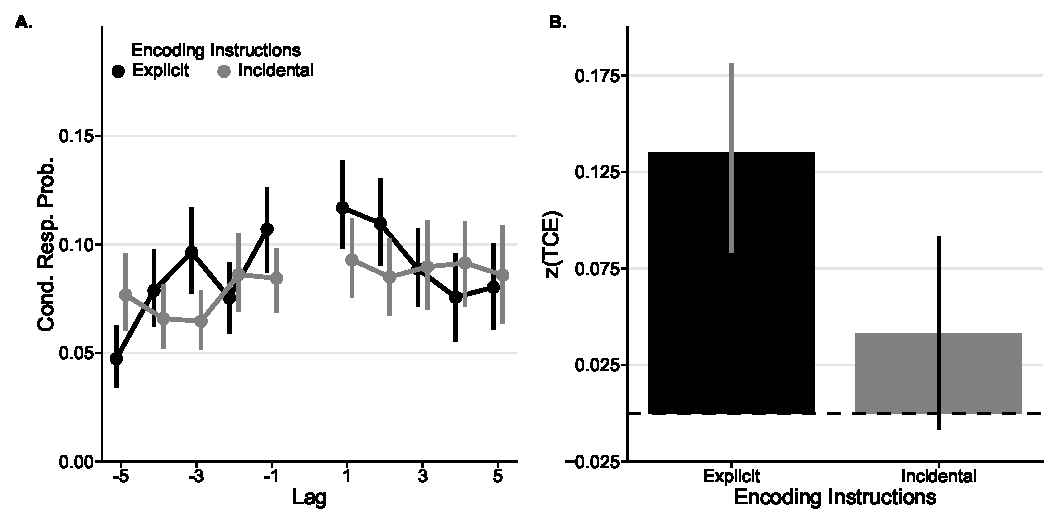
\includegraphics{figures/E1_crp_list1.pdf}
\caption{The temporal contiguity effect (TCE) on the first list under explicit versus incidental encoding using the Shoebox task (Experiment 1). \paneltext}
\label{e1_l1_crp}
\end{figure}





\color{red}
\label{TODO-5}
It is notable that even in the Explicit condition, the TCE was small compared to most previous work. Across a range of variations of the free recall task, the lag-CRP typically peaks at about 0.3--0.5 \citep{HealKaha17} compared to approximately 0.12 for the Explicit condition. The critical difference is likely amount of task experiece. In a multi-list explict encoding study \citet{HealKaha17} found that on a participant's very first list the lag-CRP peaked at approximatley 0.15 but that on the twelfth list, it peaked at 0.3. Figure~\ref{e1_l2_crp} shows the TCE for the second list in the current study. In both conditions the Z(TCE) is significant and higher than on list 1 (TODO: STATS). The TCE is, however, still lower in the Incidental than the Explicit condition prerhaps refelecting that the Explicit condition are profiting form the explicit encoding practice they gained on the first list. These finding would be difficult to account for with most existing models, because they have no mechanism simulate practice or otherwise allow contiguity to change dramatically with task experience.

%#####################
%####### E1l2 CRP ####
%#####################
\begin{figure}
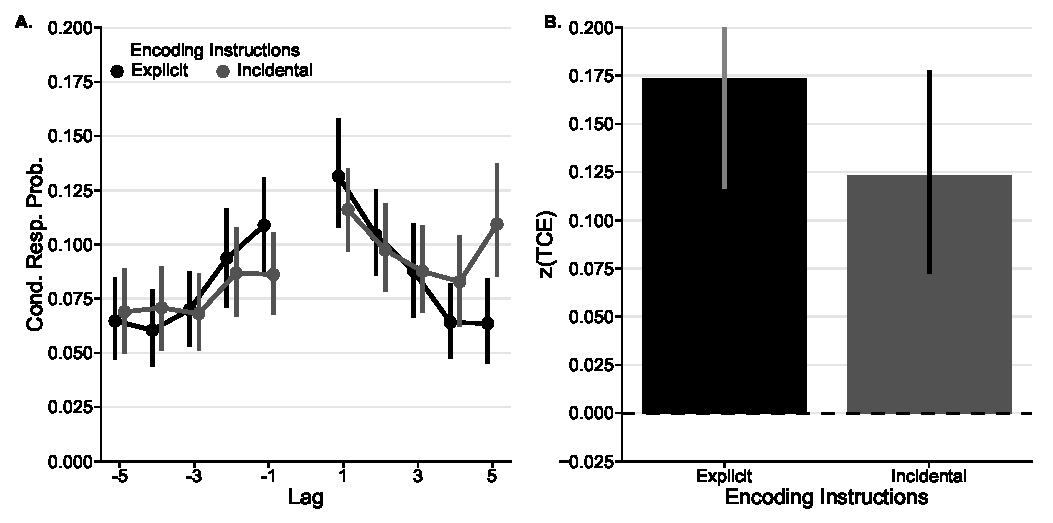
\includegraphics{figures/E1_crp_list2.pdf}
\caption{The temporal contiguity effect (TCE) on the second list under explicit versus incidental encoding using the Shoebox task (Experiment 1). \paneltext}
\label{e1_l2_crp}
\end{figure}

\color{black}


\color{red}
\label{TODO-6}
Althought the TCE is our main focus, examining other aspects of recall dynamics may help shed light on why TCE varies across conditions. Overall recall probability (Table~\ref{sampsize_table}) was lower in the Incidental condition, espically for early output positions (see A for Serial Position Curves).  This is largely attributable to Participants in the Incidental condition recalling fewer items from early serial positions  (Figure~\ref{e1_l1_spc}A). Both groups show considerable recency despite the incidental encoding and a delayed test (SPC ANOVA?) \citep[for a similar findings see][]{MarsWerd72,Neat93,GlenEtal80}.

%#####################
%####### E1l1 SPC ####
%#####################
\newcommand\spcpaneltext{All Error bars are bootstrapped within-subject 95\% confidence intervals.}
\begin{figure}
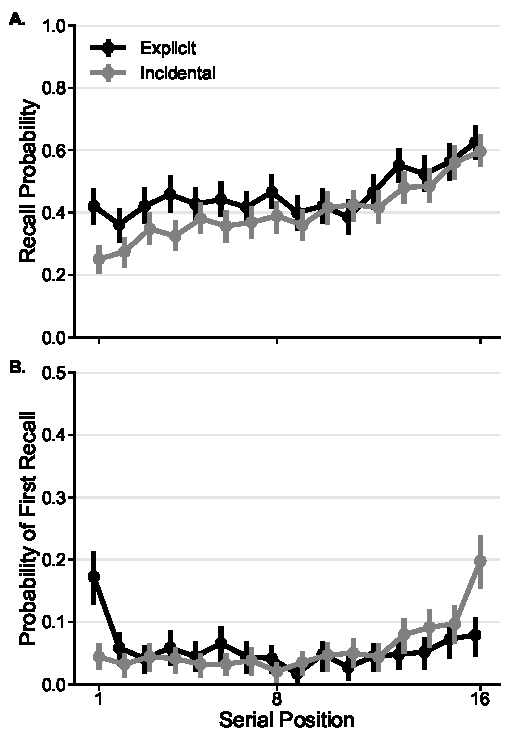
\includegraphics{figures/E1_spc_list1.pdf}
\caption{(A) Serial Position Curves and (B) Probability of First Recall curves on the first list under explicit versus incidental encoding using the Shoebox task (Experiment 1). \spcpaneltext}
\label{e1_l1_spc}
\end{figure}

In multi-list delayed free recall tasks, participants typically initiate recall by first retreiving an item from near the begining of the list \citep[i.e., they focus first on primacy items][]{ref}. Participants in the Explicit condition showed this typicla pattern, but participants in the Incidental condition showed the oppsite pattern of focusing first on recency items (Figure~\ref{e1_l1_spc}B), which is more typical of imediate recall \citep{ref}. On the second list, when everyone expected a memory test, these group differences in recall initiation and accuracy were eliminated Figure~\ref{e1_l2_spc}. 

Differences in recall dynamics between incidental and explicit encoding may be due to removing the inputus to rehershe \citep{MarsWerd72,Neat93,GlenEtal80}, which is known to increase primacy by effectively increasing the  functional serial position of early list items \citep{WARD,LAM}. But what about the TCE? Rehershal could increase TCE by causing the participants to hold adjecent items in mind at the same time \cite{HINTsaythis?}. Although the TCE has been found under conditions designed to minimize rehershal \citep{REC}, reduced rehershal may be one factor contributing to a diminished TCE under incidental encoding. 

%#####################
%####### E1l2 SPC ####
%#####################
\begin{figure}
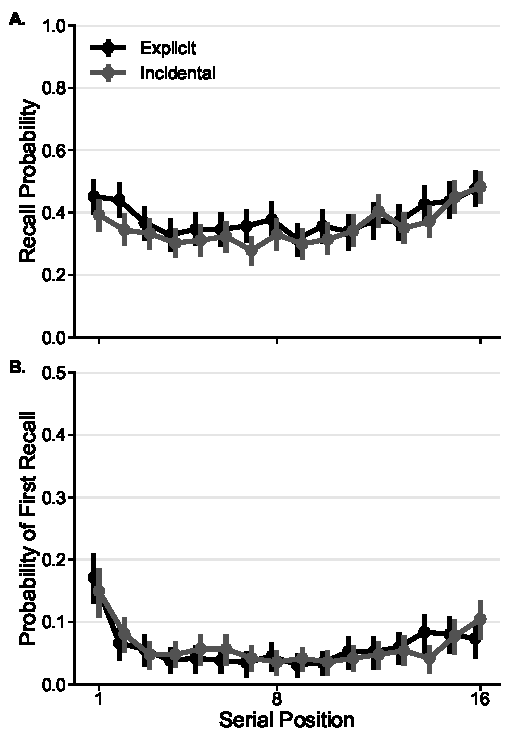
\includegraphics{figures/E1_spc_list2.pdf}
\caption{(A) Serial Position Curves and (B) Probability of First Recall curves on the second list under explicit versus incidental encoding using the Shoebox task (Experiment 1). \spcpaneltext}
\label{e1_l2_spc}
\end{figure}

In summary, Experiment 1 directly compared Explicit and Incidental encoding conditions and found that removing the intent to encode dramatically reduced the TCE. \color{black} But because the TCE has proven to be so robust in previous studies \citep{HealKaha17}, we attempt to replicate the finding in Experiment 2 using a slightly different processing task.




\section{Experiment 2}
\section{Method}

The methods were identical to those used in Experiment 1 except for the judgment task instructions (see Table 1 for sample size information).

The processing required by the Shoebox Task from Experiment 1 is quite simple. So simple that one could argue it is  ineffective at forming strong memories, which may artificially reduce the TCE. Therefore, we wanted to retain the basic task of judging size while increasing memory performance in the Incidental condition. That is, can processing that promotes memory do so without producing substantial contiguity? Mental imagery and self-referential processing are two effective ways to improve memory. Thus, the Front Door Judgment task asked subjects to imagine trying to move the object referred to by each item through the front door of their house and decide whether or not it would be possible (again, subjects were asked to indicate if this judgment was easy or difficult to make by pressing ``Y'' or ``N''). See the Supplemental Materials for the exact task instructions.

\section{Results and Discussion}
As predicted, the Front Door Task substantially improved memory accuracy in the Incidental condition. In fact, probability of recall was equal in the Explicit and Incidental conditions (Table 1) \color{red} and the differrences in Serial Position and Probability First Recall curves were reduced (Figure~\ref{e2_l1_spc}). Together, these findings suggest factors that influence memory accuracy, like rehershal, played less of a role in this Experiment.

%#####################
%####### E2l1 spc ####
%#####################
\begin{figure}
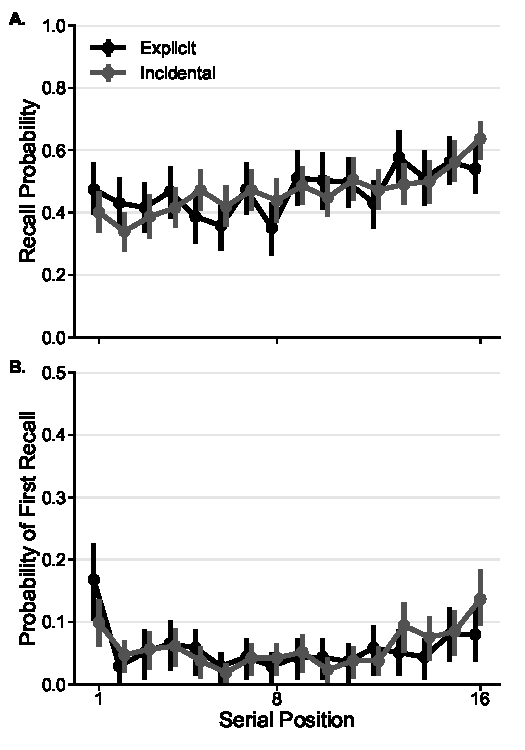
\includegraphics{figures/E2_spc_list1.pdf}
\caption{(A) Serial Position Curves and (B) Probability of First Recall curves on the first list under explicit versus incidental encoding using the Front Door task (Experiment 2). \spcpaneltext}
\label{e2_l1_spc}
\end{figure}

\color{black}

Nonetheless, the Front Door task did not produce a significant TCE under incidental encoding: Figure~\ref{e2_l1_crp} shows that whereas the Explicit condition \color{red} had a \label{done-11} Z(TCE) significantly above zero \color{black}, the Incidental condition showed a flattened lag-CRP and a Z(TCE) for which the confidence interval included zero. \color{red} Analyses of list 2, which are reported in the Supplemental Materials for this and subsequent experiemnts, replicated the Experiment 1 finding of increased contiguity. \color{black}

These results confirm that incidental encoding can \st{eliminate} \color{red} dramatically reduce \color{black} temporal contiguity without substantially decreasing memory performance \citep{NairEtal17}. This lack of coupling between level of recall and level of temporal contiguity has important theoretical implications, which we will consider in the discussion.

%#####################
%####### E2l1 crp ####
%#####################
\begin{figure}%[hp]
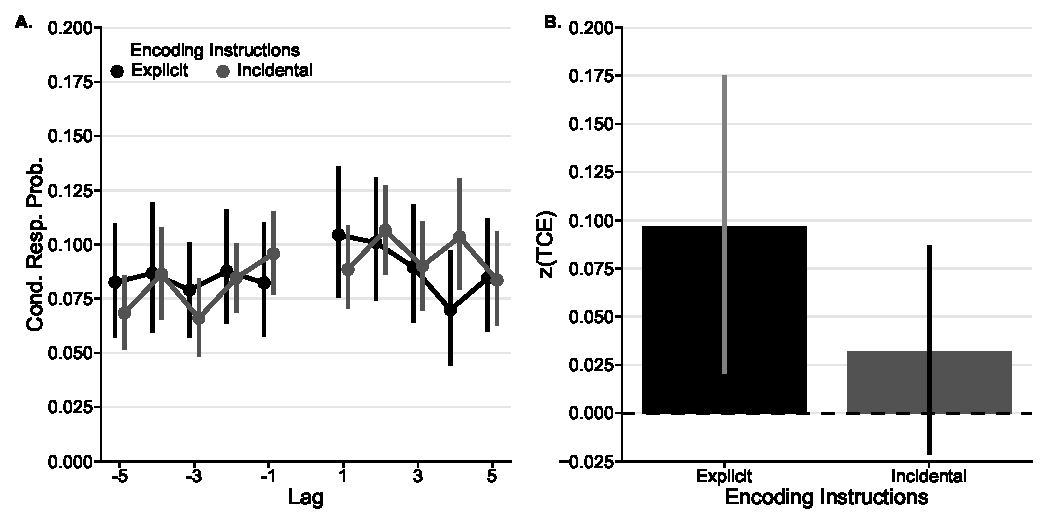
\includegraphics{figures/E2_crp_list1.pdf}
\caption{The temporal contiguity effect (TCE) on the first list under explicit versus incidental encoding using the Front Door task (Experiment 2). \paneltext}
\label{e2_l1_crp}
\end{figure}




\st{\section{Interim Discussion}}
\st{Experiments 1 and 2 show that the TCE can be absent when intent to encode is absent} \color{red} Experiments 1 and 2 show that when intent to encode is absent, the TCE is reduced to the point of being statistically indistinguishable from zero \color{black} . This result is consistent with theories that ascribe the TCE to strategic control processes. Under this interpretation, the contiguity-generating processes are more or less inseparable from the intent to encode. But is intent to encode truly necessary to find a TCE? Perhaps not. 

\color{red}
Studies showing memory for serial order after incidental learning strongly suggest that participants have access to the temporal information required to produce a TCE \cite{Nair,neat}.\color{black} \st{An alternate interpretation is that automatic encoding processes do produce contiguity but their effect is obscured by processes required by the judgment task.}  \color{red} Why do they fail to use it? In the final 2 experiments I consider two explinations. Experiment 3 tests the possibility that the details of the incidental encoding task determines wheter or not temporal contiguity influences memory search. Experiment 4 tests the possibility that temporal information \emph{is} in fact encoded incidental learning but not automatically used during memroy search. 



\section{Experiment 3}
Experiment 3 focuses on the possibility that temporal information is encoded autimaticall, but its influence is obscured by processes required by the judgment task.\color{black}~For example, many models produce a TCE because the representations of items studied close together are more similar to each other than they are to representations of items studied far apart. The Shoebox and Front Door tasks encourage subjects to maintain a common mental representation (e.g., image of a shoebox) throughout the list presentation. If this representation is incorporated into the representations of list items, it would increase the similarity of items separated by distant lags, attenuating the TCE. When effortfully memorizing, subjects likely process items in ways that are not necessary of the judgment task, perhaps decreasing the similarity of items separated by distant lags, increasing the TCE. That is, the judgment task might decrease the TCE in a way that is not due to the lack of intent to encode.

More generally, if intentional control processes are required to produce contiguity, it should be challenging, perhaps impossible, to observe a TCE under incidental encoding. But if control processes simply moderate the effect of automatic contiguity-generating processes (sometimes attenuating the TCE, sometimes accentuating it), it should be easy to find incidental encoding tasks that produce a TCE. Experiment 3 tests these predictions by examining five different encoding tasks.

\section{Method}
The methods were identical to those used in Experiment 2 except for the judgment task instructions (see Table 1 for sample size information).

The question is no longer whether explicit encoding produces a larger TCE than incidental encoding, but rather whether the TCE can ever be observed under incidental encoding. Thus, in Experiment 3 all subjects were given incidental encoding instructions, but were randomly assigned to one of five different judgment tasks that varied in the type of processing required. Otherwise, the methods were identical to those used in Experiments 1 and 2 (see Table 1 for sample size information).

\subsection{Processing Task Manipulation}
In all conditions, subjects were asked to make a judgment about each word as it was presented. Here, we describe the type of processing that each task was intended to discourage (or encourage). Again, to allow for the same yes/no response for each task, subjects were asked to indicate if the judgment was easy to make under the guise of norming the items for a later study. See the Supplemental Materials for the exact task instructions.



\subsubsection{Weight Task} The Weight Task was similar to the size judgment tasks used in the first two experiments except that it asked subjects to compare each item's \emph{weight} to a common referent: a bottle of water. Specifically, they were asked to judge whether each word referred to an object that was heavier than ``a standard bottle of water you'd purchase from a vending machine''. Because weight is not an easily visualizable attribute, the Weight Task might be expected to reduce the likelihood that subjects will maintain the same vivid mental image throughout the list. Thus, it may produce a larger TCE if associating each item with a common mental image tends to attenuate the TCE.

\subsubsection{Animacy Task} The Animacy Task asks subjects whether each item refers to an object that is living or non-living. Like the Shoebox, Front Door, and Weight tasks, the Animacy task requires subjects to consider only a single attribute of each item (i.e., animacy status). But unlike the aforementioned tasks, it does not provide a reference object against which to compare each item. Thus, it further reduces the likelihood of maintaining a single vivid image throughout the list. 

\subsubsection{Moving Scenario Task} The Moving Scenario Task asks subjects to judge the relevance of each word to a scenario: moving to a foreign land \citep{NairEtal17}. Subjects are likely to maintain some representation of this scenario across items, but because it does not specify any pre-existing dimension, like size or weight, each item may be expected to activate many different attributes, lowering the similarity of mental representations from item to item.

\subsubsection{Movie Task} The instructions for the Movie Task explain that ``when you read a word, it can trigger many different thoughts'' and gives the example of the word baseball triggering a series of thoughts: ``you might have a mental image of a baseball, you might hear the crack of a bat hitting a ball, you might think of related concepts like ballpark, players, and fans...''. It then asks subjects to allow each item ``to activate as many different thoughts as possible. Then use these thoughts to generate a mental movie (like a detailed image of spending an afternoon at a baseball game or what it is like to be a player on a baseball field).'' Subjects then judge whether or not it was easy to form such a mental movie. This tasks removes the requirement to consider each item along the same dimensions and instead encourages subjects to think deeply about the unique attributes of each item, which might be expected to cause very different mental representations to be activated with each successive item, perhaps increasing the TCE \citep[for a different prespective on the influence of item specific processing on the TCE, see][]{McDaEtal11}. 

\subsubsection{Relational Task} The Relational Task is similar to the Movie Task except instead of being asked to make a new mental movie for each item, subjects are asked to ``try to incorporate each new word into your existing mental movie. For example, if the next word was ``owner'', you should allow it to activate many associated thoughts and then incorporate it into your existing ``ballpark'' movie.'' This condition, which is similar to deep encoding strategies free recall subjects often adopt spontaneously \citep{DelaKnow05}, encourages subjects to notice semantic associations between temporally proximate items. As such, it is much like the ``reminding'' process \cite{Hint16} suggested contributes to the TCE \citep[for a similar manipulation see][]{BowClar69}. Thus, this condition should maximize the chance of observing a TCE. 

\color{red}
\subsubsection{Varying Size Task} This task was similar to the Shoebox task from Experiment 1 with three exceptions. First, instead of judging every word aginst a common referent (a shoebox), a different referent was randomly selected for each word (see the appendix for a full list of referents). Instead of deciding if the presented word would ``fit in'' the referent, participants were asked if the word was ``larger than'' the referent (e.g., AFRICA: "Is it easy to judge if it is larger than a Golf Ball"). Third, because the changing referent made the task more complex, each word was presented for 5 sec (as opposed to the 4 second presentation rate of all other conditions)
\color{black}

\section{Results and Discussion}

\color{red}
The five encoding tasks produced considerabl variation in recall accuracy (Table 1) as well as differrences in Serial Position and Probability First Recall curves (Figure~\ref{e3_l1_spc}). Most notably, whereas the first 4 tasks produced SPCs and PFRs similar to those of the incidental encoding conditions of the first two experiments, the Relational Task produced a SPC and a PFR that more closley resembles those seen in multi-trial delayed recall. This suggests that the Relational Task sucesfully mimiced some features of intentional encoding.

%#####################
%####### 3l1 spc ####
%#####################
\begin{figure}
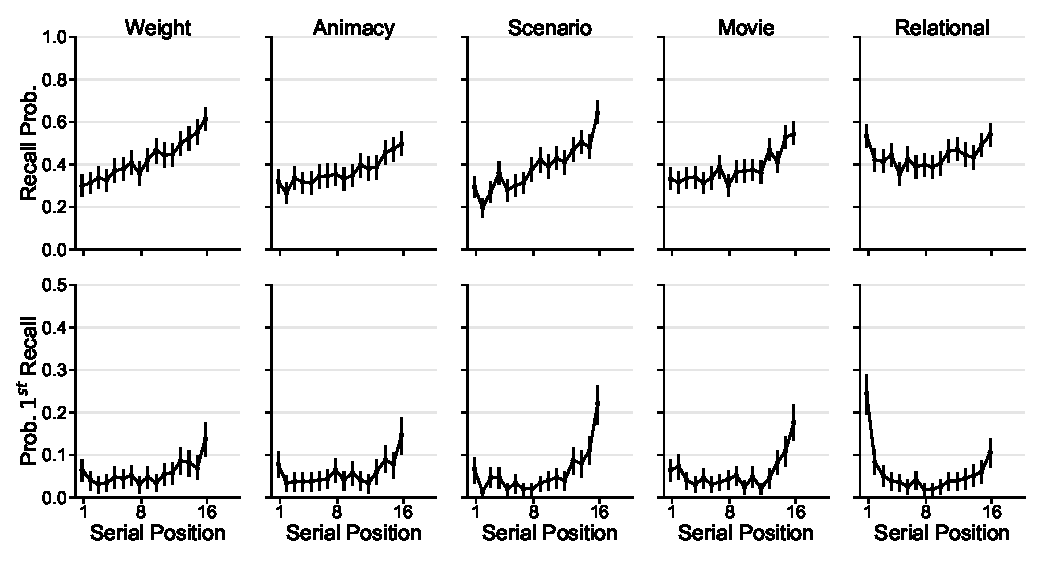
\includegraphics{figures/E3_spc_list1.pdf}
\caption{(Top row) Serial Position Curves and (Bottom row) Probability of First Recall curves on the first list under incidental encoding with different judgment tasks (Experiment 3). \spcpaneltext}
\label{e3_l1_spc}
\end{figure}

\color{black}

\st{As seen in Figure 3,} \color{red} Critically, \color{black}~all of the processing tasks produced a TCE under incidental encoding conditions \color{red}(Figure~\ref{e3_l1_crp})\color{black}. For each task, the lag-CRP tends to decrease with increasing $|lag|$ and the Z(TCE) is significantly above zero. These results show that although the TCE can be attenuated under incidental conditions (as in Experiments 1 and 2), the lack of intent to encode, per se, does not eliminate contiguity. 

Indeed, perhaps the most remarkable feature of the data is how little the size of the TCE differs among the tasks, consistent with the suggestion that the TCE is due to automatic encoding processes. The only condition for which the z(TCE) differed significantly from any other condition was the Relational Task condition, which asked subjects to integrate each item in to an ongoing movie \footnote{The Relational Task also increased recall relative to most of the other tasks (see Table 1), which replicates \citet{BowClar69}}. This suggests that encouraging subjects to notice semantic similarities among items does indeed enhance temporal contiguity \citep{Hint16}, at least under incidental encoding conditions. 

\st{It is also notable that there is substantial variation in recall levels across conditions (see Table 1) despite modest variation in the TCE, which is consistent with Experiments 1, 2 and Nairne et al. (2017). We return to this point in the General Discussion.}

\st{Finally, we note} \color{red}It should be noted \color{black} that although Experiments 1 and 2 conceptually replicated Nairne et al.'s (2017) finding of no contiguity under incidental encoding using different encoding tasks, Experiment 3 failed to replicate the finding using an encoding task (Moving Scenario Task) almost identical to Nairne et al.'s. \st{This failure may be due to our larger sample size ($n=299$ here versus $N=80$ in E1 and $N=80$ in E2 of Nairne et al.) providing more power to detect a small contiguity effect combined with seemingly minor methodological differences (e.g., different list lengths and presentation rates). In any case,} \color{red}Nonetheless, \color{black}~the message across the present three experiments is consistent with Nairne et al.'s findings: incidental encoding \emph{can} \st{eliminate contiguity and it certainly} reduce the size of the effect relative to explicit encoding \color{red} without substantially reducing recall accuracy\color{black}. 

\color{red}
The failure to exactly replicate the Nairne et al. (2017) null finding may be due to a larger sample ($n=299$ here versus $N=80$ in E1 and $N=80$ in E2 of Nairne et al.) providing more power to detect a small contiguity effect. But this raises the possibility that even the current Experiments 1 and 2 were underpowered as well. Although sample sizes were selected to provide enought power to detect effects smaller than those typiucally reported, as discussed above, the observed effects were much smaller than the typical effect in multi-list studies. Indeed comparing the significant effects in Figure~\ref{e3_l1_crp} with the non-significant effects in Figures~\ref{e1_l1_crp}~and~\ref{e2_l1_crp}, shows that they all of similar magnitude---of the 7 incidental encoding conditions reported across the three figures, only the Relation Task condition is significantly different from any other (TODO:STATS). Across these conditions the average effect size was TODO:COHEN. In the final experiment, we used larger samples to ensure we could detect effects of this magnitude. (TODO:POWER ANA)

\color{black}

%#####################
%####### 3l1 crp ####
%#####################
\begin{figure}%[hp]
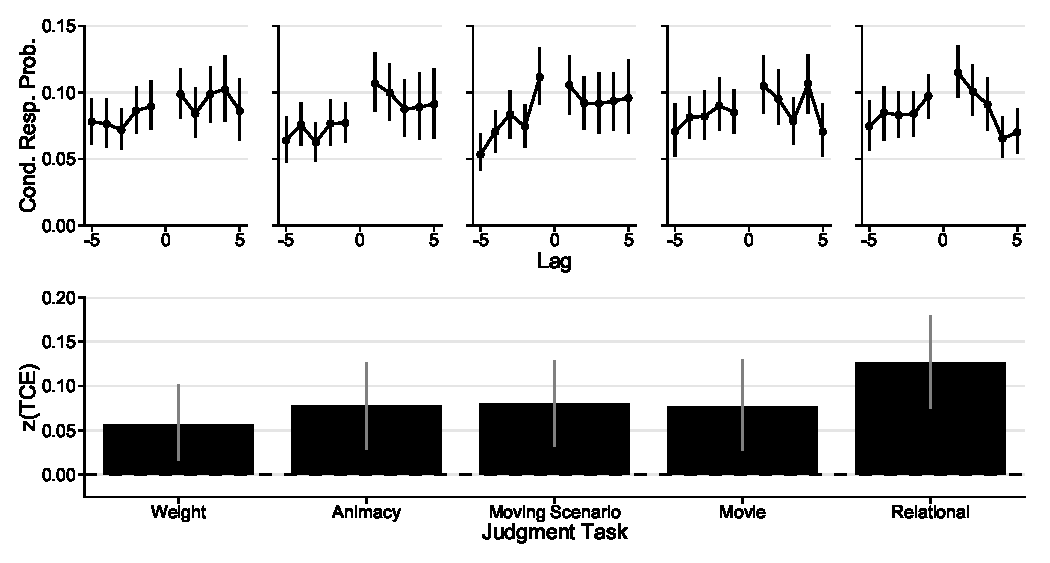
\includegraphics{figures/E3_crp_list1.pdf}
\caption{The temporal contiguity effect (TCE) on the first list under incidental encoding with different judgment tasks (Experiment 3). (Top) Lag-conditional response probability functions. Error bars are bootstrapped within-subject 95\% confidence intervals. (Bottom) The average Z(TCE).  Error bars are bootstrapped between-subject 95\% confidence intervals. Z(TCE) for a given subject is computed as follows: An observed temporal factor score was computed as the average percentile ranking the temporal lag of each actual transition in the recall sequence with respect to the lags of all transitions that were possible at that time. To determine the temporal factor score expected by chance, a permutation distribution was created by randomly shuffling the order of recalls within the sequence 10,000 times and computing a temporal factor score for each shuffling. The reported value, Z(TCE), is z-score of the observed temporal factor score within the permutation distribution.}
\label{e3_l1_crp}
\end{figure}


\color{red}
\section{Experimet 4}


The TCE is the observation that the order in which events are experienced has a powerful infleunce on the order in which those events are recalled. The first 3 experiments place an important cavet on this general observation: when the events are experneced without expectation of a memory test, the influence of order of experience on order of recall can be dramatically reduced. These findings have important theoritical implications, espicially for models of memroy in which the same mechanisms are responsible for both recall accuracy and TCE and therefore have difficulty accounting for succesfull recall in the absence of temporal contiguity. The final experiment attempts to clarify the theoritical implications of this cavet by answering two questions.

First, do incidental encoding tasks completely eleminate the TCE, or do they leave a small resudual TCE which can be detected with sufficient statistical power? Second, is the reduced TCE due to a total failure to encode temporal information or is it due to a failure to adopt a strategy of using memory search? 



\section{Method}
The study phase was identical to that used in the Varying Size task of Experiment 3 except the size referent was always a shoebox.

For the recall phase participants in the Free Recall Condition were given the same recall instructions used in Experiments 1--3. Participants in the Serial Recall Phase were given same instructions with one additional sentence: ``Try to recall the words in the <\textbf{same order you saw them}'' (including the bold emphasis). 

\label{TODO-8} add demographic info
For this experiment participants studied and recalled only a single list. This change provided extra time for a short demographic questionaire at the end of the study. Participants (XX male and XX female; see Table 1) had average XXX.

\section{Results and Discussion}

Recall accuracy (Table 1) was lower in the Serial Recall condition than the Free Recall condition. Serial Recall produced more primacy than the Free Recall, as is visiable in both the SPC and the PFR (Figure~\ref{e4_l1_spc}). 

\begin{figure}
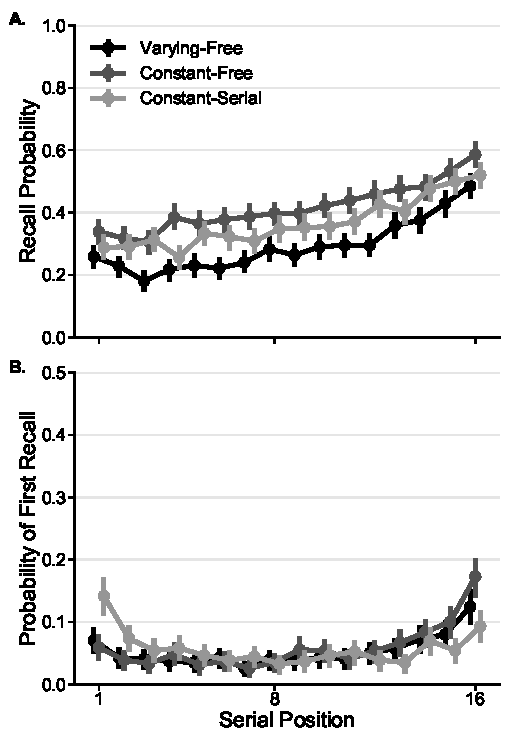
\includegraphics{figures/E4_spc_list1.pdf}
\caption{(A) Serial Position Curves and (B) Probability of First Recall curves on the first list as a function of encoding task variability and recall instructions (Experiment 4). \spcpaneltext}
\label{e4_l1_spc}
\end{figure}

Figure~\ref{e4_l1_crp} reveals that both conditions showed significant contiguity effects.

-This finding suggests that the failure to find a significant TCE in Experiments 1 and 2 may have been due to a lack of statistical power. To be clear, their is no doubt that incidental encoding can reduce the TCE to \emph{near} zero, which is a very important finding. But it is also theoritically important that a small residual TCE remains.

-The Serial Recall condition showed a larger TCE (STAT) than did the Free Recall condition, but also lower overall recall. This suggests that even after incidental encoding, temporal information is available for use in memroy search \cite{nair}, but participants rely on aditional sources of information to guide recall.



\begin{figure}%[hp]
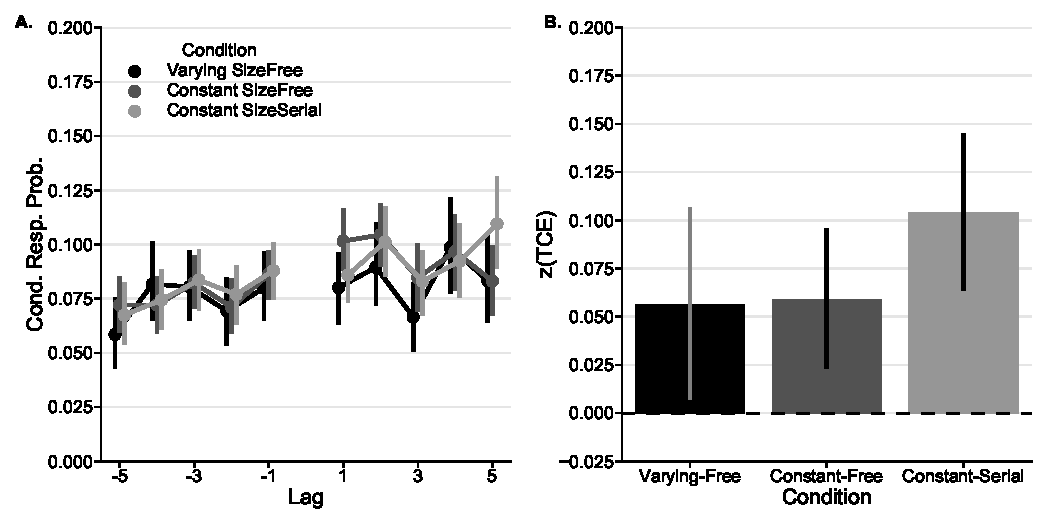
\includegraphics{figures/E4_crp_list1.pdf}
\caption{The temporal contiguity effect (TCE) on the first list as a function of encoding task variability and recall instructions (Experiment 4). \paneltext}
\label{E4_crp_list1}
\end{figure}

\color{black}





\section{General Discussion}
Does the TCE depend on control processes that implement task-specific strategies during deliberate encoding \citep{Hint16}? Or are automatic processes that operate even when we form new memories in the absence of deliberate study sufficient to produce a TCE \citep{HealKaha17}? The former possibility suggests the TCE should be easily eliminated by removing the impetus to engage controlled processes. The latter suggests the the TCE should be observable under most encoding circumstances. The data tell us that neither view is totally correct.

Experiment 3 showed that the TCE is not completely dependent on intent to encode: a robust TCE was observed in five different implicit tasks. These results provide an existence proof for temporal contiguity under incidental encoding and rule out the possibility that the TCE is an artifact of task-specific strategies implemented by controlled encoding processes. The TCE seems to arise from automatic encoding processes. The bigger contribution of these data, however, is to point out serious limitations of existing models of these automatic encoding processes. 


\begin{figure}%[hp]
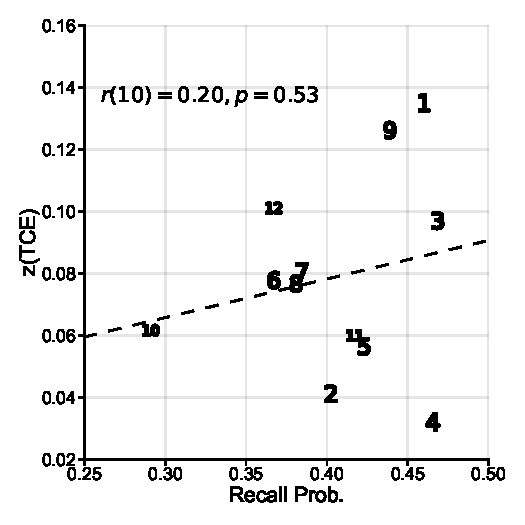
\includegraphics{figures/correlation.pdf}
\caption{The size of the temporal contiguity effect versus the overall level of recall. Each dot represents the average of one of the conditions 13 conditions reported across the 4 experiments.}
\label{corr}
\end{figure}

Experiments 1 and 2 showed that intent to encode matters a great deal: in these experiments, the TCE was eliminated when controlled encoding processing was discouraged via incidental encoding instructions and particular types of processing were encouraged by the judgment task. This finding points to a gap in our understanding of how encoding processes influence contiguity. There have been few attempts to model how automatic memory processes interact with controlled processes to meet task demands \citep{LehmMalm13,PolyEtal09}, thus existing models would likely have difficulty accounting for the difference between Explicit and Incidental conditions. The challenge is avoiding adding a homunculus to the models that does the hard work of translating task instructions into changes in encoding processes. What computational mechanisms allow instructions to regulate encoding processes?

Equally important is the finding that variations in the size of the TCE are not tightly coupled with variations in overall recall levels. Figure 4 plots level of recall versus level of TCE across all conditions from Experiments 1, 2, and 3. \label{done-12} \color{red} The correlation is quite small and non-significant \color{black} suggesting that recall success may depend less on temporal contiguity than has been suggested by analyses of individual differences in free recall of explicitly encoded lists \citep{SedeEtal10,HealEtal14}. Indeed, some of the conditions with the highest recall levels had the lowest levels of contiguity. This is most dramatically illustrated in Experiment 2 where both conditions showed the same level of recall, but only the Explicit condition showed a significant TCE. This finding may pose a challenge for models that assume episodic memory for an event is fundamentally mediated by its associations to a context representation that changes across time \citep[e.g.,][]{LohnEtal14,HealKaha15}. 

The precise nature of the relationship between time and context drift in these models points to a possible answer to this challenge. Although the change in context from time $t$ to time $t+lag$ is correlated with the passage of time, it is not \emph{driven} by time in most versions of the model \citep[but see][for a model in which drift is driven by time]{HowaEtal14a}. Instead, context drift is driven by the cognitive representations activated by external and internal events. As a result, the similarity of the context representation, $\mathbf{c}_t$, at time $t$ to the context representation at some other time, $\mathbf{c}_{t+lag}$, is partly a function of the similarity of the cognitive representations activated by the events that intervene between $t$ and $t+lag$. Under some incidental encoding tasks, the cognitive representations activated by successive items are likely to be similar, causing context to drift slowly and resulting in a shallow contiguity effect. By contrast, if subjects are intending to encode items for a memory test they are likely to engage in elaborative processing which might cause context to drift rapidly and produce a steeper contiguity effect. A critical question for modelers then, is whether existing models can use differential drift rates to capture the large difference in TCE between Incidental and Explicit conditions while simultaneously capturing the near equal levels of recall.

In summary, these results show that control processes are not necessary to produce a TCE, but that they can powerfully influence the size of the effect and even eliminate it. Thus, the results point to serious limitations in existing theories of TCE---we understand much about how memory encoding processes produce temporal contiguity, but we understand little about how these processes are controlled.

\bibliography{healey_lab}
\end{document}